%---------------------------------------------------
% Nombre: capitulo1.tex  
% 
% Texto del capitulo 1
%---------------------------------------------------

\chapter{Aplicaci�n de texturas}

En esta tercera pr�ctica no hay necesidad de modelar nada con blender sino que nos centraremos en aplicar texturas para que los modelos anteriores se asimilen m�s a la realidad. En la primera parte \ref{parte1} se pide aplicar la textura de la tierra a una esfera y la de un dado a un cubo. En la segunda parte \ref{parte2} de la pr�ctica se aplicar�n texturas sobre el modelo realizado en la pr�ctica anterior, en nuestro caso el robot de la saga \textit{Star Wars}, R2D2, que podemos ver de nuevo en la figura \ref{img_1}.

\begin{figure}[H]
	\centering
		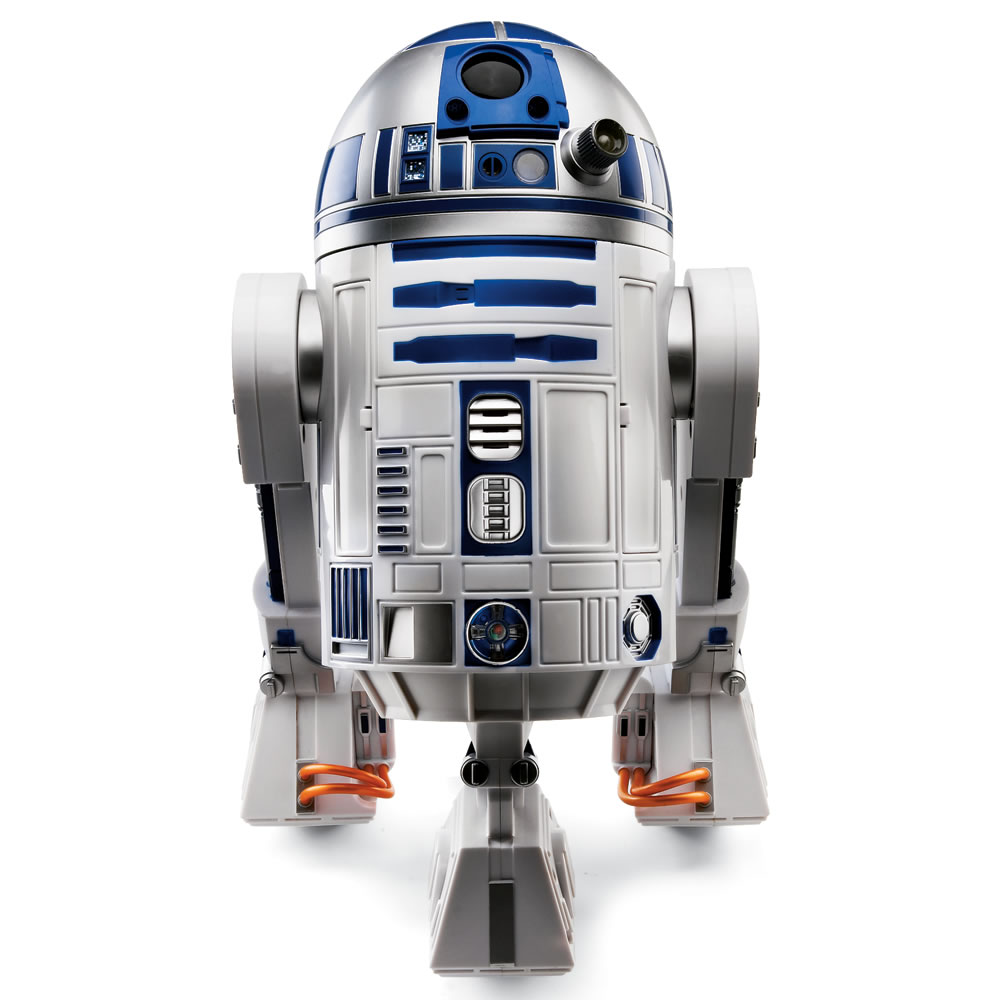
\includegraphics[scale=0.2]{./Capitulo1/Imagenes/r2d2.jpg}
		\caption{Modelo R2D2.}
	\label{img_1}
\end{figure} 


\section{Texturas del globo terraqueo y el dado}
\label{parte1}

Los modelos est�n a�adidos a la entrega de la pr�ctica pero no se detalla su realizaci�n ya que ha sido siguiendo el tutorial did�ctico \cite{1} que el profesor ofrece para la realizaci�n ambos. El resultado del dado podemos verlo en la figura \ref{img_2} y el globo terr�queo en la figura \ref{img_3}.

\begin{figure}[H]
	\centering
		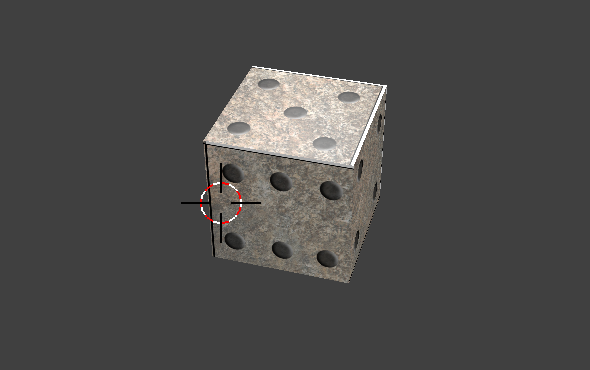
\includegraphics[scale=0.6]{./Capitulo1/Imagenes/2.png}
		\caption{Dado.}
	\label{img_2}
\end{figure} 

\begin{figure}[H]
	\centering
		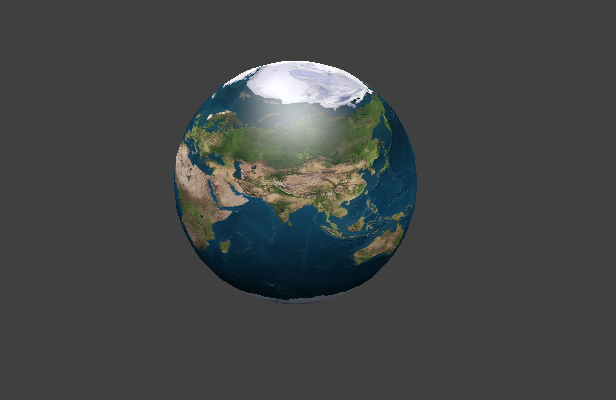
\includegraphics[scale=0.6]{./Capitulo1/Imagenes/3.png}
		\caption{Globo terr�queo.}
	\label{img_3}
\end{figure} 

La realizaci�n de la esfera es muy sencilla y la del dado, es algo m�s compleja ya que implica el uso de costuras, aunque hay tutoriales que explican el proceso de selecci�n de las mismas \cite{2}.   

\section{Texturas del robot}
\label{parte2}

Para aplicar texturas sobre el robot hemos tenido que buscar algunas que se adapten bien al mismo. Aunque el robot R2D2 puede encontrarse en multitud de versiones en internet, es complicado encontrar una textura que se adapte completamente al mismo, finalmente nos hemos decantado por la textura que podemos encontrar en la figura \ref{img_4}. Esta textura la iremos descomponiendo en diversas texturas para  ir aplicando cada lugar al respectivo espacio del modelo. 


\begin{figure}[H]
	\centering
		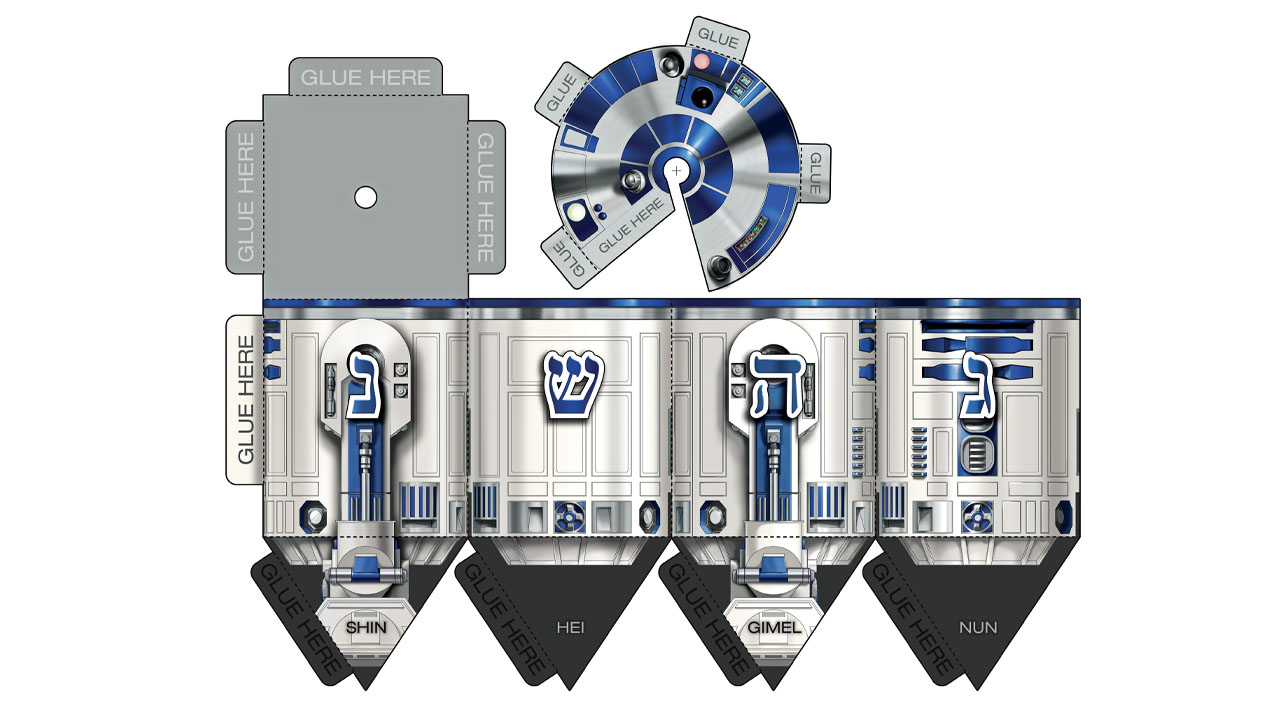
\includegraphics[scale=0.3]{./Capitulo1/Imagenes/4.png}
		\caption{Textura utilizada para el modelo.}
	\label{img_4}
\end{figure} 

\subsection{Cabeza}

Para aplicar texturas a la cabeza hemos seguido los siguientes pasos. Primero hemos editado la imagen en \ref{img_4} en Photoshop para quedarnos solo con la parte de textura (eliminamos las partes del recortable) y rellenar el hueco de en medio, ya que sino se ver�a negro al no haber textura. 

El siguiente paso, nos aseguramos de tener desactivada la opci�n de \textbf{limit selection to visible} y con  \textbf{control + B} seleccionamos la parte superior de la esfera que corresponde con la cabeza de nuestro modelo. Tenemos que haber generado una nueva pantalla de tipo \textbf{UV/Image Editor} tras lo cual abriremos la imagen de la cabeza del robot. Una vez hecho esto, en el �rea de modelado 3D pulsaremos sobre  \textbf{Mesh > UV/Unwrap>Unwrap } tras lo que tendremos lo que podemos ver en la figura \ref{img_5}.


\begin{figure}[H]
	\centering
		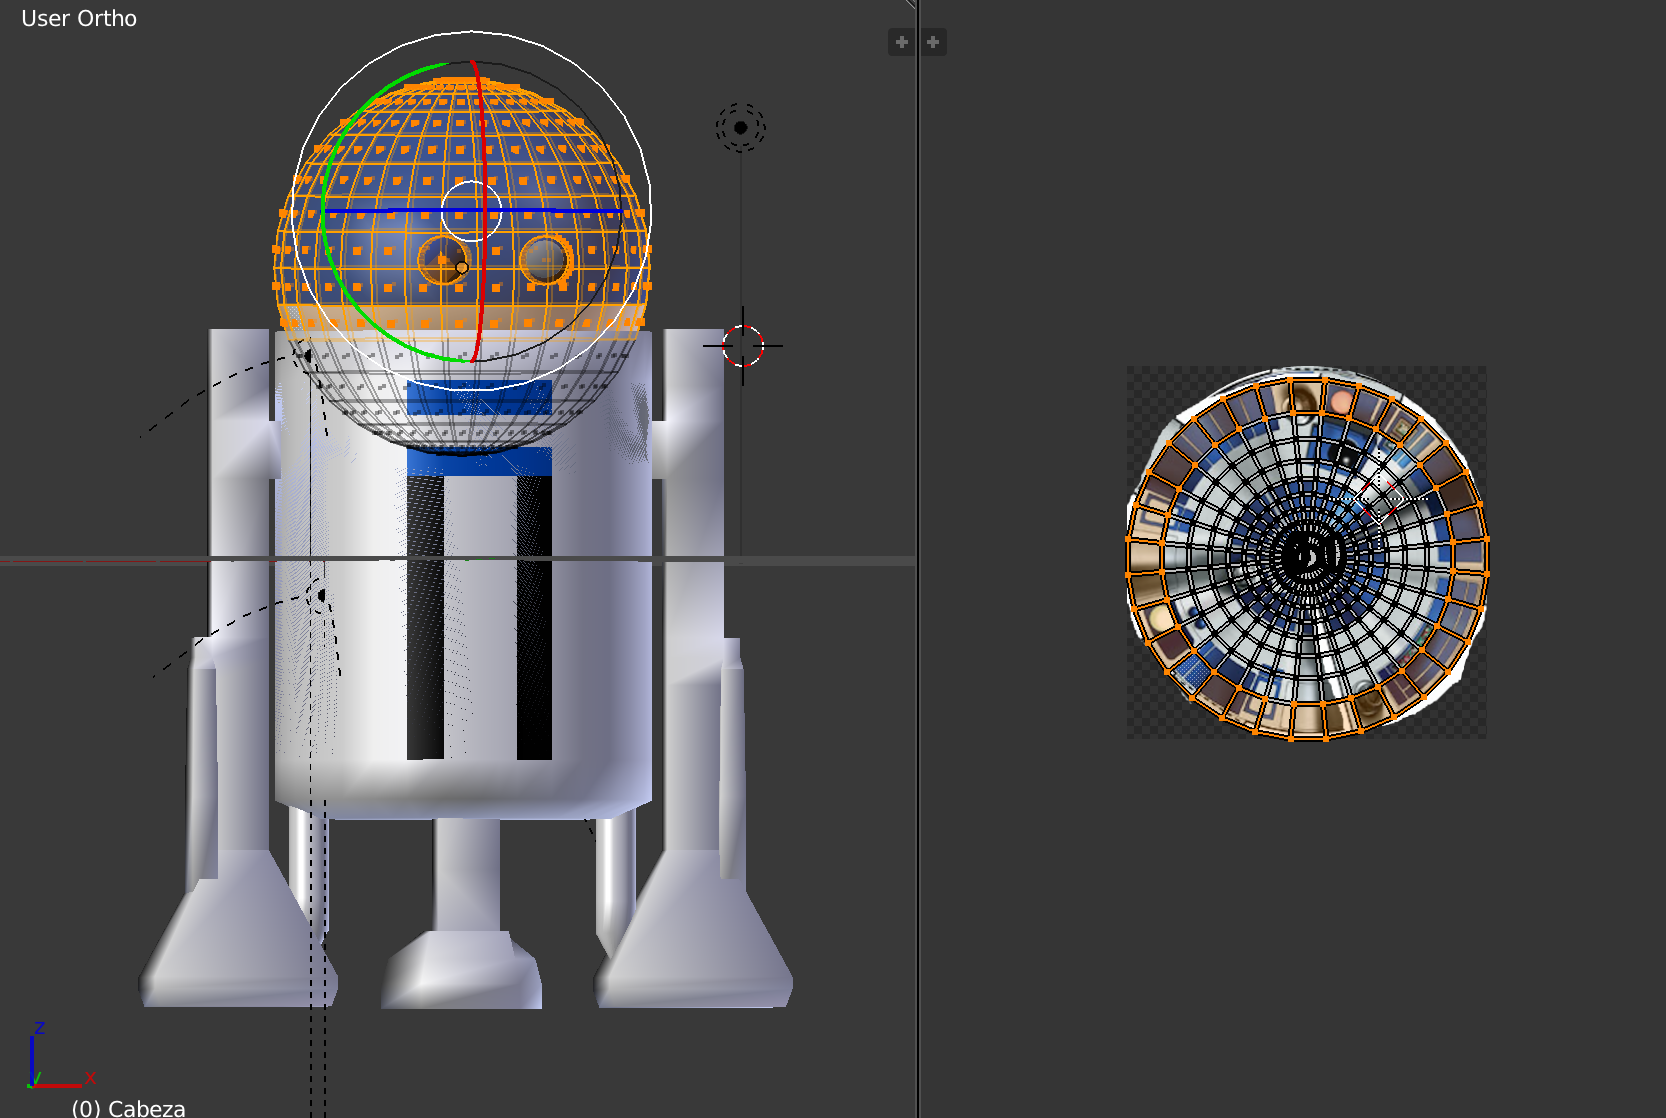
\includegraphics[scale=0.4]{./Capitulo1/Imagenes/5.png}
		\caption{Textura de la cabeza.}
	\label{img_5}
\end{figure} 


Para aplicar la textura en el �rea bajo Scene, podremos encontrar la zona de materiales. Solo tendremos que a�adir un nuevo material, asignarlo y marcar la opci�n \textbf{FaceTextures}, tras lo cual tendremos la textura asignada. Para ver como queda, podremos pasar la escena a \textbf{Render}, y por medio de rotaciones y traslaciones en la proyecci�n de la imagen la ubicaremos donde necesitemos para que se adapte a la realidad.  


\subsection{Cuerpo}

Para aplicar la textura al cuerpo seguiremos el mismo proceso que para la cabeza. Seleccionamos el cilindro del cuerpo, y de nuevo en  \textbf{Mesh > UV/Unwrap } aunque esta vez seleccionaremos \textbf{Cilynder Projection} lo que facilita enormemente el trabajo. Tras Esto por medio de los atajos \textbf{g} y \textbf{s} para transformaciones tendremos algo como en la figura \ref{img_6}


\begin{figure}[H]
	\centering
		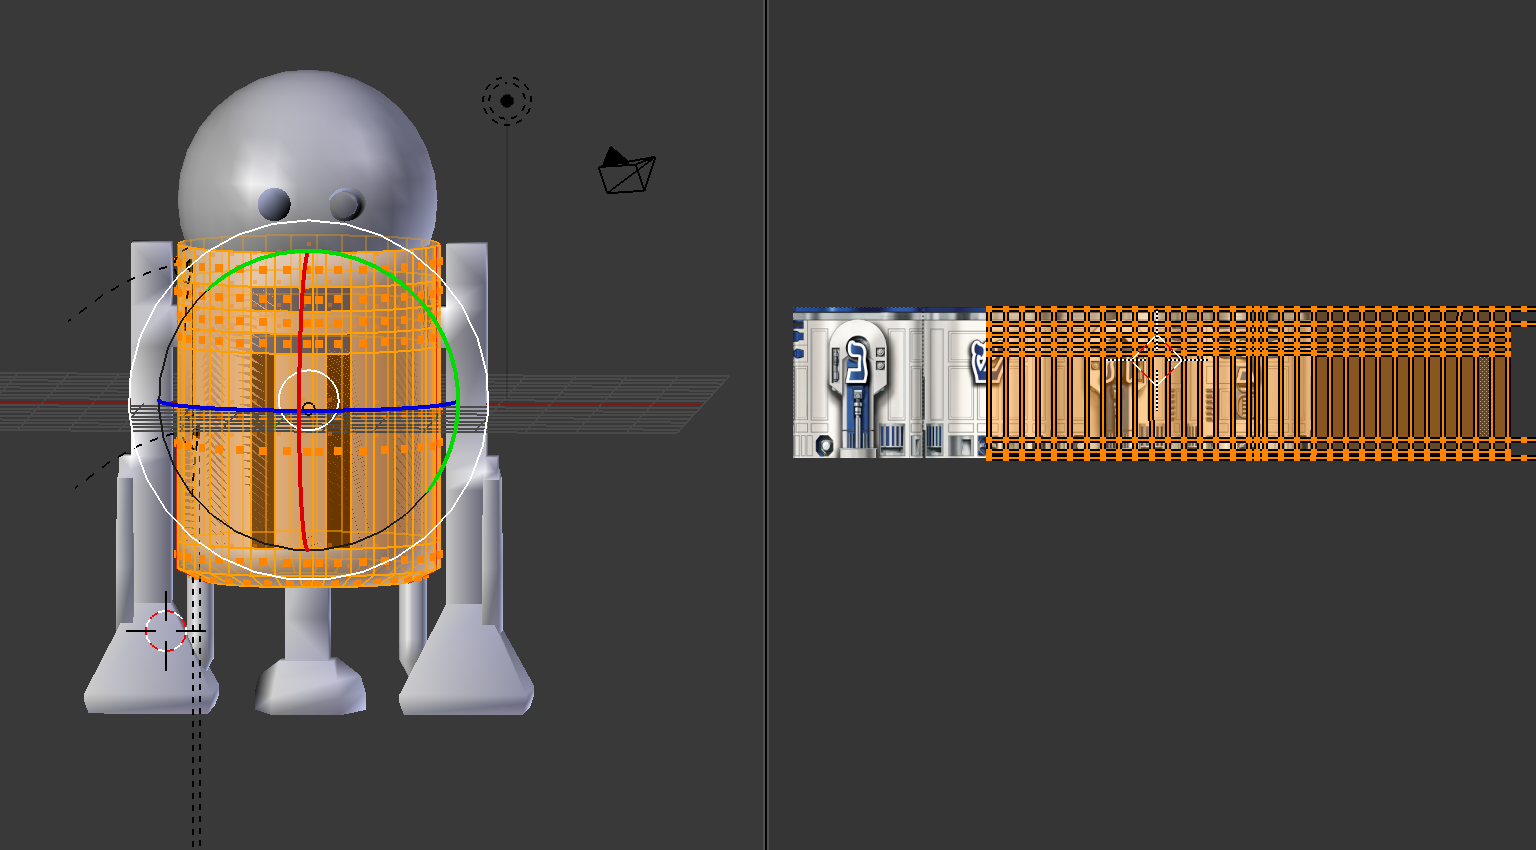
\includegraphics[scale=0.4]{./Capitulo1/Imagenes/6.png}
		\caption{Textura del cuerpo.}
	\label{img_6}
\end{figure} 

\subsection{Extremidades}

Las extremidades cuentan de diversas texturas diferentes en funci�n de si estamos en el lado derecho o izquierdo por problemas de simetr�a. Por tanto, se ha obtenido del modelo visto en la figura \ref{img_4} ademas de otra vista por internet los distintos componentes y con el proceso estudiado en las secciones anteriores hemos ido asignando manualmente cada cara a su parte de la textura como puede verse en la figura \ref{img_7}.


\begin{figure}[H]
	\centering
		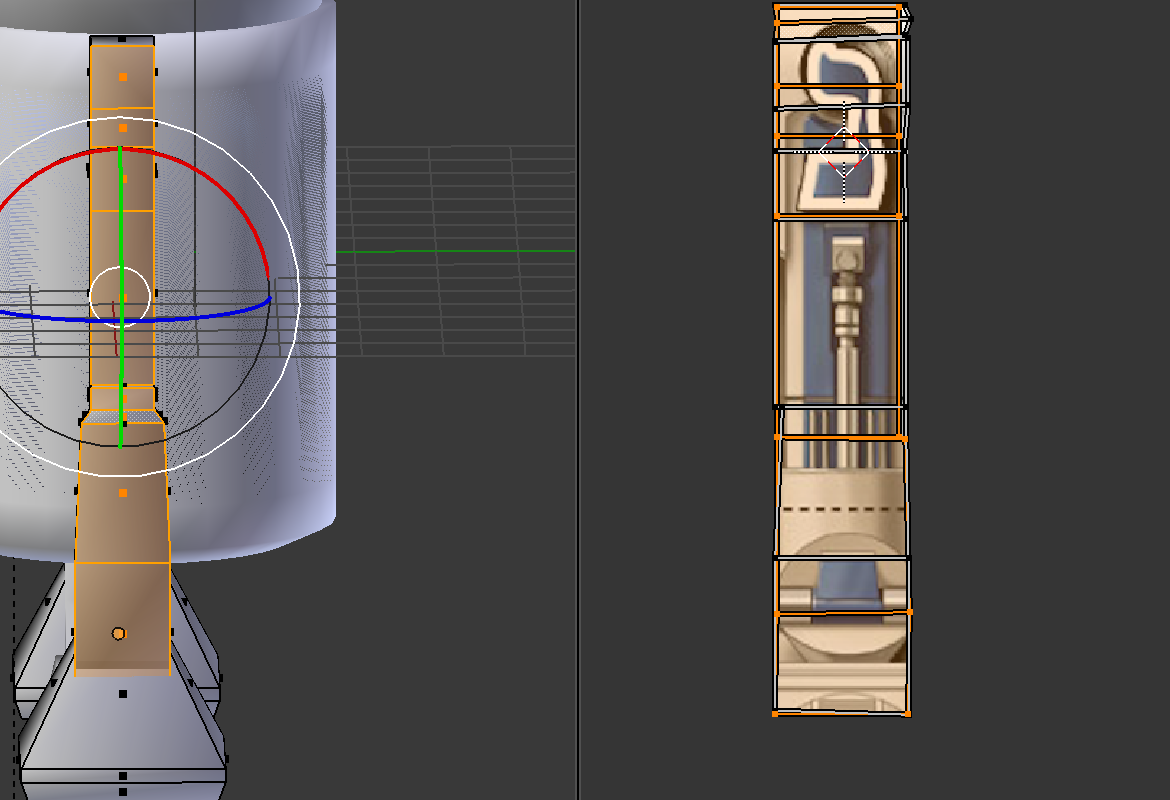
\includegraphics[scale=0.4]{./Capitulo1/Imagenes/7.png}
		\caption{Texturas en las extremidades.}
	\label{img_7}
\end{figure} 

Las cadenas o pies del robot han sido texturizadas a mano, seleccionando cada uno de los v�rtices y movi�ndolos hasta que se adapten a la imagen cargada tal y como vemos en la figura \ref{img_8}.

\begin{figure}[H]
	\centering
		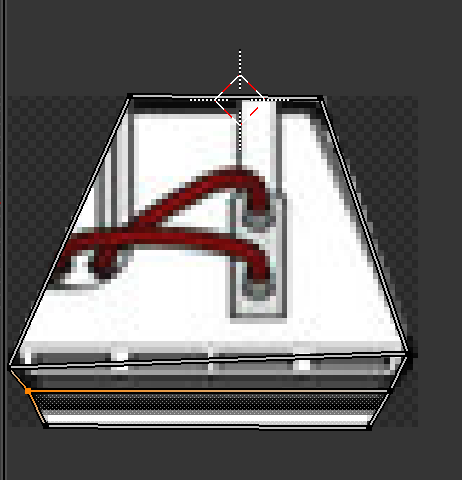
\includegraphics[scale=0.4]{./Capitulo1/Imagenes/8.png}
		\caption{Textura en las cadenas.}
	\label{img_8}
\end{figure} 


\subsection{Modelo final}

El modelo final con todas las texturas a�adidas puede verse en la figura \ref{img_9}.

\begin{figure}[H]
	\centering
		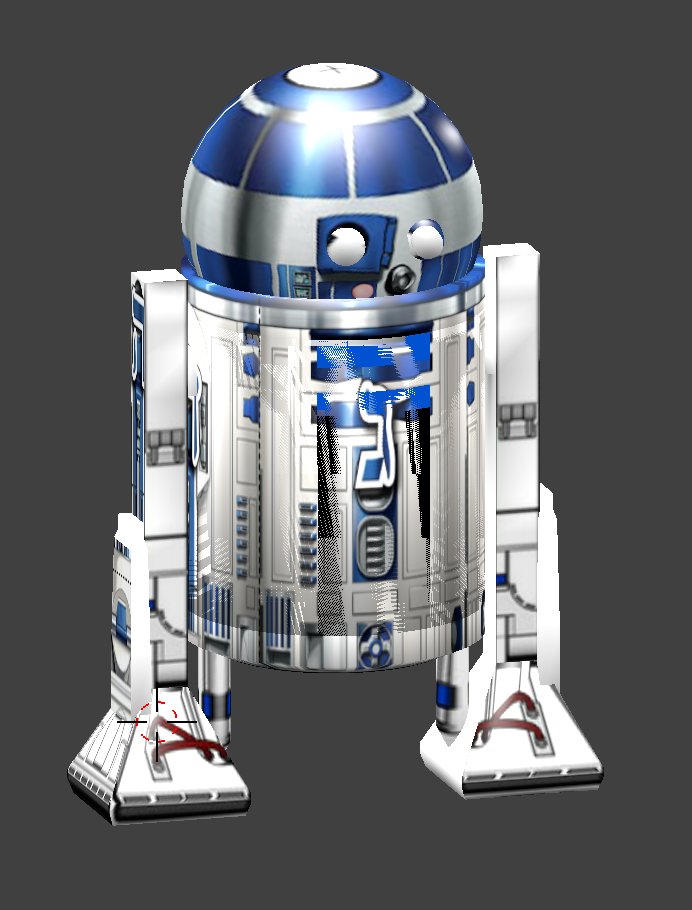
\includegraphics[scale=0.4]{./Capitulo1/Imagenes/9.png}
		\caption{Modelo final con todas las texturas.}
	\label{img_9}
\end{figure} 


\section{Conclusiones}

Es interesante ver como teniendo la imagen apropiada, o sin tenerla pero teniendo experiencia con las costuras, es muy sencillo el aplicar texturas sobre un modelo cualquiera. Esto nos da una imagen m�s clara a�n si cabe de la potencia Blender a la hora de desarrollar modelos 3D que se asemejen a la realidad, alejandose mucho de la tediosa labor de realizarlo a bajo nivel como por ejemplo con OpenGL. 

\clearpage
%---------------------------------------------------